\documentclass{article}

\title{Programmazione di Sistema: OS Internals}
\date{2022-09-28}
\author{Manuel Cadeddu}
\usepackage[italian]{babel}
\usepackage{amsmath}
\usepackage{graphicx}
\usepackage{subcaption}
\usepackage{setspace}
\usepackage{xcolor} 


\begin{document}
	\pagenumbering{arabic}
	\maketitle
	\newpage
	\doublespacing
	\tableofcontents
	\singlespacing
	\newpage
	
	\section{Main Memory}

		\subsection{Introduzione}

			\subsubsection{Hardware di Base}
				La Memoria consiste in un array di byte identificati da un indirizzo. 
				\\La CPU può accedere solamente alla \textbf{Memoria Centrale} (RAM) e ai \textbf{Registri}, ma non al \textbf{Disco}. Quindi, tutte le istruzioni in esecuzione e i dati che utilizzano devono essere caricati in Memoria prima che la CPU possa operare su essi.
				\\I Registri hanno una memoria molto piccola e veloce ed è possibile accedervi con un solo colpo di clock. Invece, per accedere alla Memoria sono necessari più colpi di ck e questo può causare \textit{stalli}. Per migliorare la situazione sono state introdotte le \textbf{Cache}: buffer di memoria veloce che si trovano nel processore e permettono di non accedere in memoria (se possiedono i dati cercati).
				\\Un problema da gestire è quello di permettere ad un processo di accedere solo alla memoria per la quale è autorizzato. Per farlo si usano solitamente implementazioni hw, perché il SO non interviene negli accessi della CPU alla memoria per motivi di prestazioni.
				\\Una tecnica per implementare questa protezione è quella di avere due registri nella CPU: il \textbf{Base Register} e il \textbf{Limit Register}. Il Base Register contiene l'indirizzo minimo accedibile dal processo, il Limit Register la porzione di memoria assegnata al processo e, insieme, definiscono lo spazio degli \textit{Indirizzi Logici}. Quando la CPU deve accedere alla memoria verifica che l'indirizzo sia compreso tra il Base e Base + Limit. Se un processo cerca di accedere a un indirizzo non valido, viene generata una \textit{trap} che restituisce il controllo al SO per gestirla.
				\begin{figure}[ht!]
					\centering{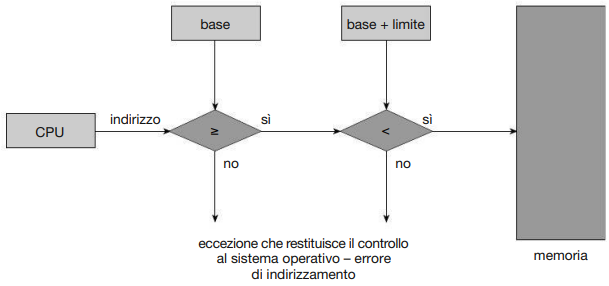
\includegraphics[width=12cm,height=5cm,keepaspectratio]{ch9_1.png}}
				\end{figure}
				\\I Base e Limit Register sono modificabili solo tramite \textit{istruzioni privilegiate} che possono essere eseguite solo in modalità kernel e, poiché solo il SO può essere eseguito in tale modalità, i processi utente non possono modificare il loro valore.

			\newpage
			\subsubsection{Fasi di Elaborazione di un Programma}
				Vediamo i vari componenti che permettono ad un file sorgente di diventare un eseguibile e di essere caricato in RAM per essere eseguito:
				\begin{itemize}
					\item \textbf{preprocessore}: spesso considerato parte del compilatore, permette l'inclusione di header files, di espandere macro, di eseguire compilazione condizionale\dots 
					\\In output si ha un altro file C;
					\item \textbf{compilatore}: traduce il C in linguaggio macchina e produce un \textit{file oggetto} per ogni file C;
					\item \textbf{linker}: unisce i file oggetto e le librerie statiche per creare un \textit{file eseguibile} (\textit{loadable image});
					\item \textbf{loader}: copia la \textit{loadable image} in Memoria, connettendola con librerie dinamiche.
				\end{itemize}
				\begin{figure}[ht!]
					\centering{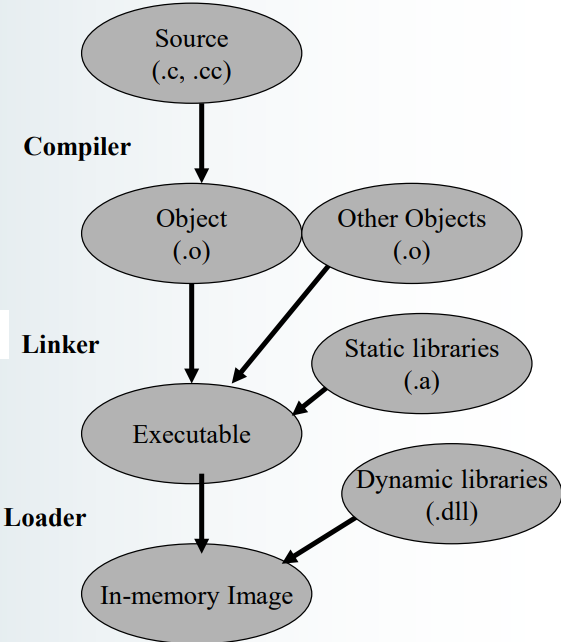
\includegraphics[width=12cm,height=5.5cm,keepaspectratio]{ch9_2.png}}
				\end{figure}
			
			\subsubsection{Address Binding}
				L'Address Binding si rifferisce alla mappatura delle istruzioni e dei dati in posizioni di memoria fisica.
				\\Generalmente, gli indirizzi nel file sorgente sono simbolici (es. nomi variabili), il compilatore associa questi indirizzi simbolici a indirizzi rilocabili (es. 14 byte dall'inizio di questo modulo) e, infine, il linker o il loader genera gli indirizzi assoluti (es. 7014 byte dall'inizio della memoria). Ogni associazione rappresenta una corrispondenza da uno spazio d'indirizzi a un'altro.
				\\Esistono tre tipi di address binding:
				\begin{itemize}
					\item \textbf{Compile Time Address Binding}: se il compilatore sa dove il processo risiederà in memoria, può generare \textbf{codice assoluto}. In questo caso, se dovesse cambiare la locazione iniziale, bisognerebbe ricompilare il codice;
					\item \textbf{Load Time Address Binding}: se in fase di compilazione non è possibile sapere in che punto della memoria risiederà il processo, il compilatore genera \textbf{codice rilocabile}. In questo caso il \textit{codice assoluto} viene generato in fase di caricamento e, se cambia l'indirizzo del processo, è sufficiente ricaricare il codice per ottenere il nuovo indirizzo "base";
					\item \textbf{Execution Time Address Binding}: se durante l'esecuzione il processo può essere spostato in memoria, si deve ritardare la generazione degli \textit{indirizzi assoluti} fino alla fase di esecuzione. La maggior parte dei SO usa questa soluzione.
				\end{itemize}
		
			\subsubsection{Spazi di Indirizzi Logici e Fisci}
				Un indirizzo generato dalla CPU è normalmente chiamato \textbf{indirizzo logico}, mentre quello caricato nel rigistro dell'indirizzo di memoria è chiamato \textbf{indirizzo fisico}.	
				\\I metodi di associazione degli indirizzi in fase di compilazione e di caricamento producono indirizzi logici e fisici identici. Con l'associazione in fase di esecuzione gli indirizzi logici non coincidono con quelli fisici. In questo caso ci si riferisce agli indirizzi logici col termine \textbf{indirizzi virtuali}.
				\\L'insieme degli indirizzi logici generati da un programma è lo \textbf{spazio degli indirizzi logici}; l'insieme degli indirizzi fisici corrispondenti a tali indirizzi logici è lo \textbf{spazio degli indirizzi fisci}.
				\\Per implementare l'Execution Time Address Binding,  l'associazione dagli indirizzi virtuali a quelli fisici è svolta da un dispositivo (interno alla CPU) detto \textbf{MMU} (\textbf{Memory Management Unit}). Come vedremo più avanti, questo binding può essere realizzato in diversi modi. Per esempio, sommando l'indirizzo logico al contenuto del registro base (ora chimato \textbf{relocation register}).
				\begin{figure}[ht!]
					\centering{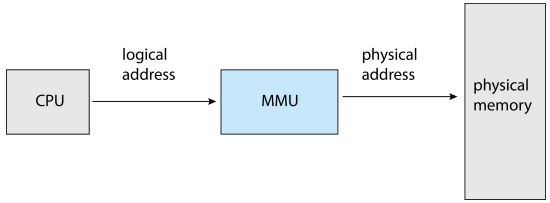
\includegraphics[width=12cm,height=3.5cm,keepaspectratio]{ch9_3.png}}
				\end{figure}

			\subsubsection{Dynamic Loading}
				Nella discussione svolta fin’ora, era necessario che l’intero programma e i dati di un processo fossero presenti nella memoria fisica perché il processo potesse essere eseguito. Per migliorare l’utilizzo della memoria si può ricorrere al \textbf{caricamento dinamico} (dynamic loading), mediante il quale si carica una procedura solo quando viene richiamata; tutte le procedure si tengono su disco in un formato di caricamento rilocabile. Si carica il programma principale in memoria e quando una procedura deve richiamarne un’altra, controlla innanzitutto che sia stata caricata. Se non è stata caricata, caricare in memoria la procedura richiesta e aggiornare le tabelle degli indirizzi del programma. A questo punto il controllo passa alla procedura appena caricata.
				\\Il caricamento dinamico non richiede un supporto particolare del SO. Spetta agli utenti progettare i programmi in modo da trarre vantaggio da un metodo di questo tipo. Il SO può tuttavia aiutare il programmatore fornendo librerie di procedure che realizzano il caricamento dinamico.
			

			\subsubsection{Dynamic Linking e Librerie Condivise}
				Le \textbf{Dynamically Linked Libraries} (\textbf{DLLs}, librerie caricate dinamicamente) sono librerie di sistema che vengono collegate ai programmi utente quando questi vengono eseguiti. Alcuni SO consentono solo il collegamento statico (static linking), in cui le librerie di sistema sono trattate come qualsiasi altro modulo oggetto e combinate dal caricatore nell’immagine binaria del programma. Il concetto di linking dinamico, invece, è analogo a quello di dynamic loading. Invece di differire il caricamento di una procedura fino al momento dell’esecuzione, si differisce il collegamento. Questa caratteristica si usa soprattutto con le librerie di sistema, per esempio le librerie di subroutine del linguaggio. Senza questo strumento tutti i programmi di un sistema dovrebbero disporre, all’interno dell’eseguibile, di una copia della libreria di linguaggio (o almeno delle procedure cui il programma fa riferimento). Tutto ciò spreca spazio nei dischi e in memoria centrale.
				\\Con il linking dinamico, invece, per ogni riferimento a una procedura di libreria s’inserisce all’interno dell’eseguibile una piccola porzione di codice di riferimento (\textbf{stub}), che indica come localizzare la giusta procedura di libreria residente in memoria o come caricare la libreria se la procedura non è già presente. Durante l’esecuzione, lo stub controlla se la procedura richiesta è già in memoria, altrimenti provvede a caricarla; in entrambi i casi lo stub sostituisce se stesso con l’indirizzo della procedura, che viene poi eseguita. In questo modo, quando si raggiunge nuovamente quel segmento del codice, si esegue direttamente la procedura di libreria, senza costi aggiuntivi per il linking dinamico. Con questo metodo tutti i processi che usano una libreria del linguaggio eseguono la stessa copia del codice della libreria. Questo sistema è noto anche con il nome di \textbf{librerie condivise}.
				\\A differenza del caricamento dinamico, il linking dinamico e le librerie condivise richiedono generalmente l’assistenza del sistema operativo. Se i processi presenti in memoria sono protetti l’uno dall’altro, il sistema operativo è l’unica entità che può controllare se la procedura richiesta da un processo è nello spazio di memoria di un altro processo, o che può consentire l’accesso di più processi agli stessi indirizzi di memoria.

		\subsection{Allocazione Contigua della Memoria}
			La memoria centrale deve contenere sia il SO che i vari processi, quindi bisogna gestirla in modo efficiente. Vediamo ora la prima tecnica per l'allocazione della memoria: l'\textbf{allocazione contigua della memoria}.
			\\La RAM viene di solito divisa in due partizioni, una per il SO e una per i processi. Poiché l'IVT si trova solitamente agli indirizzi inferiori, anche il SO viene allocato agli indirizzi più bassi.
			\\Con l’allocazione contigua della memoria, ciascun processo è contenuto in una singola sezione di memoria contigua a quella che contiene il processo successivo. Per assicurarsi che si acceda alla memoria corretta è possibile utilizzare i registri Base e Limit:
			\begin{figure}[ht!]
				\centering{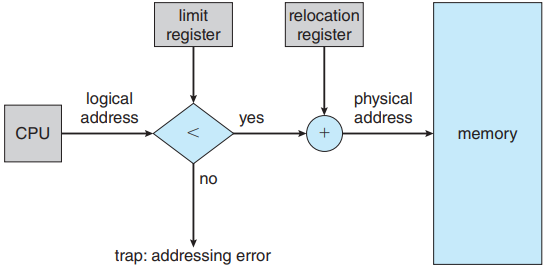
\includegraphics[width=12cm,height=4cm,keepaspectratio]{ch9_4.png}}
			\end{figure}
			\\L'utilizzo di questi registri può risultare util anche per cambiare dinamicamente la dimensione della memoria dedicata al processo (non sempre possibile).

			\subsubsection{Allocazione della Memoria}
				Uno dei metodi più semplici per l’allocazione della memoria consiste nel suddividere la stessa in partizioni di dimensione fissa.
				\\Nello schema a partizione variabile il SO conserva una tabella in cui sono indicate le partizioni di memoria disponibili e quelle occupate. Inizialmente
				tutta la memoria è a disposizione dei processi utenti; si tratta di un grande blocco di memoria disponibile, un buco (\textbf{hole}). Nel lungo periodo la memoria contiene una serie di buchi di diverse dimensioni.
				\begin{figure}[ht!]
					\centering{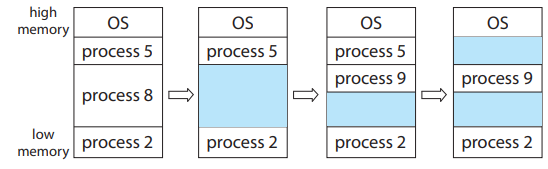
\includegraphics[width=12cm,height=3cm,keepaspectratio]{ch9_5.png}}
				\end{figure}
				\\Quando entrano nel sistema, i processi vengono inseriti in una coda d’ingresso. Per determinare a quali processi si debba assegnare la memoria, il SO tiene conto dei requisiti di memoria di ciascun processo e della quantità di spazio di
				memoria disponibile. Quando a un processo si assegna dello spazio, il processo stesso viene caricato in memoria e può quindi competere per il controllo della CPU. Al termine, rilascia la memoria che gli era stata assegnata, e il SO può impiegarla per un altro processo presente nella coda d’ingresso.
				\\I criteri più usati per scegliere un buco libero tra quelli disponibili nell’insieme sono i seguenti:
				\begin{itemize}
					\item \textbf{Firstfit}: si assegna il primo buco abbastanza grande. La ricerca può cominciare sia dall’inizio dell’insieme di buchi sia dal punto in cui era terminata la ricerca precedente. Si può fermare la ricerca non appena s’individua un buco libero di dimensioni sufficientemente grandi;
					\item \textbf{Bestfit}: si assegna il più piccolo buco in grado di contenere il processo. Si deve
					compiere la ricerca in tutta la lista, a meno che questa non sia ordinata per dimensione. Tale criterio produce le parti di buco inutilizzate più piccole;
					\item \textbf{Worstfit}: si assegna il buco più grande. Anche in questo caso si deve esaminare tutta la lista, a meno che non sia ordinata per dimensione. Tale criterio produce le	parti di buco inutilizzate più grandi, che possono essere più utili delle parti più
					piccole ottenute col criterio best-fit.
				\end{itemize}
				Con l’uso di simulazioni si è dimostrato che sia first-fit sia best-fit sono migliori rispetto a worst-fit in termini di risparmio di tempo e di utilizzo di memoria. D’altra parte nessuno dei due è chiaramente migliore dell’altro per quel che riguarda l’utilizzo della memoria ma, in genere, first-fit è più veloce.

			\subsubsection{Frammentazione}
				Si distinguono:
				\begin{itemize}
					\item \textbf{frammentazione esterna}: spazio libero in RAM tra i diversi processi;
					\item \textbf{frammentazione interna}: memoria non occupata dal processo che però è stata allocata per esso.
				\end{itemize}
				

\end{document}